\subsection{Confiabilidade e detecção de falhas}

\subsubsection{Descrição do problema e hipóteses probabilísticas}

A confiabilidade é uma preocupação central no projeto de sistemas
computacionais, pois servidores, por exemplo, podem falhar de maneira imprevisível
e a indisponibilidade tem custo elevado. O objetivo deste estudo é quantificar a
probabilidade de um sistema permanecer em funcionamento ao longo do tempo e
avaliar o ganho obtido com a redundância de componentes.

O tempo até a falha de um componente é modelado por uma variável aleatória
contínua $T$. A hipótese probabilística central é que esse tempo segue uma
distribuição exponencial de taxa $\lambda$, o que equivale a supor uma taxa de
falha constante ao longo da vida útil \cite{harcholbalter2024probability}. Essa
escolha decorre da propriedade de falta de memória apresentada na
Equação~\ref{eq:conf_memoryless}, segundo a qual
um componente que já operou por um tempo $s$ tem a mesma distribuição de vida
restante de um componente novo. A segunda hipótese é que as falhas dos diversos
componentes são independentes entre si, o que permite combinar as probabilidades
individuais por produto.

\begin{equation}
	P(T > s + t \mid T > s) = P(T > t), \qquad s, t \ge 0
	\label{eq:conf_memoryless}
\end{equation}

\subsubsection{Modelagem probabilística}

A confiabilidade de um componente é a probabilidade de ele ainda estar em
funcionamento no instante $t$, dada na Equação~\ref{eq:conf_exp}. O tempo médio
até a falha é a esperança da distribuição exponencial e vale
$1/\lambda$.

\begin{equation}
	R(t) = P(T > t) = e^{-\lambda t}, \qquad E[T] = \frac{1}{\lambda}
	\label{eq:conf_exp}
\end{equation}

Sistemas reais combinam vários componentes. Em um arranjo em série todos os
componentes precisam funcionar, de modo que o sistema falha assim que o primeiro
componente falha. Sob independência, a confiabilidade do arranjo em série é o
produto das confiabilidades, conforme a Equação~\ref{eq:conf_serie}
\cite{ross2010probabilidade}.

\begin{equation}
	R_{\text{serie}}(t) = \prod_{i=1}^{n} R_i(t)
	\label{eq:conf_serie}
\end{equation}

Em um arranjo em paralelo, ou redundante, o sistema funciona enquanto ao menos um
componente estiver operante, falhando apenas quando o último falha. A
confiabilidade é o complemento do produto das probabilidades de falha de cada
componente, conforme a Equação~\ref{eq:conf_paralelo} \cite{ross2010probabilidade}.

\begin{equation}
	R_{\text{paralelo}}(t) = 1 - \prod_{i=1}^{n} \bigl(1 - R_i(t)\bigr)
	\label{eq:conf_paralelo}
\end{equation}

\subsubsection{Implementação em R}

A confiabilidade foi estimada por simulação de Monte Carlo. Foram gerados os
tempos de vida de $100000$ sistemas, cada um com seus componentes exponenciais
independentes de taxa $\lambda = 0{,}1$, o que corresponde a um tempo médio até a
falha de $10$ por componente. O tempo até a falha de cada arranjo decorre diretamente da sua
estrutura, sendo o mínimo dos tempos no caso em série e o máximo no caso em
paralelo. O Listing~\ref{lst:conf_gera} gera os tempos de vida e os arranjos.

\begin{lstlisting}[caption={Geração dos tempos de vida e dos arranjos.}, label={lst:conf_gera}]
lambda <- 0.1
N      <- 100000
comp   <- matrix(rexp(N * 3, rate = lambda), nrow = N, ncol = 3)

vida_unico <- comp[, 1]
vida_serie <- pmin(comp[, 1], comp[, 2], comp[, 3])
vida_paral <- pmax(comp[, 1], comp[, 2], comp[, 3])
\end{lstlisting}

A confiabilidade empírica em um instante $t$ é a fração de sistemas que ainda não
falharam, conforme o Listing~\ref{lst:conf_emp}.

\begin{lstlisting}[caption={Confiabilidade empírica em função do tempo.}, label={lst:conf_emp}]
t_grid <- seq(0, 40, by = 0.5)
R_emp  <- function(vida) sapply(t_grid, function(t) mean(vida > t))
\end{lstlisting}

\subsubsection{Resultados e interpretação}

A Tabela~\ref{tab:conf_mtbf} compara o tempo médio até a falha de cada arranjo. O
arranjo em série reduz esse tempo de $10$ para cerca de $3{,}3$, pois basta uma falha
para derrubar o sistema, enquanto o arranjo em paralelo o eleva para cerca de
$18{,}3$. Em todos os arranjos a estimativa empírica difere do valor teórico
apenas na segunda casa decimal.

\begin{table}[H]
	\centering
	\caption{Tempo médio até a falha por arranjo, com $\lambda = 0{,}1$.}
	\begin{tabular}{lccc}
		\toprule
		& Único & Série de 3 & Paralelo de 3 \\
		\midrule
		Empírico & 9,9818 & 3,3173 & 18,3247 \\
		Teórico  & 10,0000 & 3,3333 & 18,3333 \\
		\bottomrule
	\end{tabular}
	\label{tab:conf_mtbf}
\end{table}

A Figura~\ref{fig:conf_curvas} mostra as curvas de confiabilidade dos arranjos
único, em série e em paralelo ao longo do tempo. Os pontos empíricos acompanham
as curvas teóricas, e a ordenação é clara, pois o arranjo em paralelo preserva
confiabilidade alta por muito mais tempo que o componente isolado, enquanto o
arranjo em série decai mais rápido.

\begin{figure}[H]
	\centering
	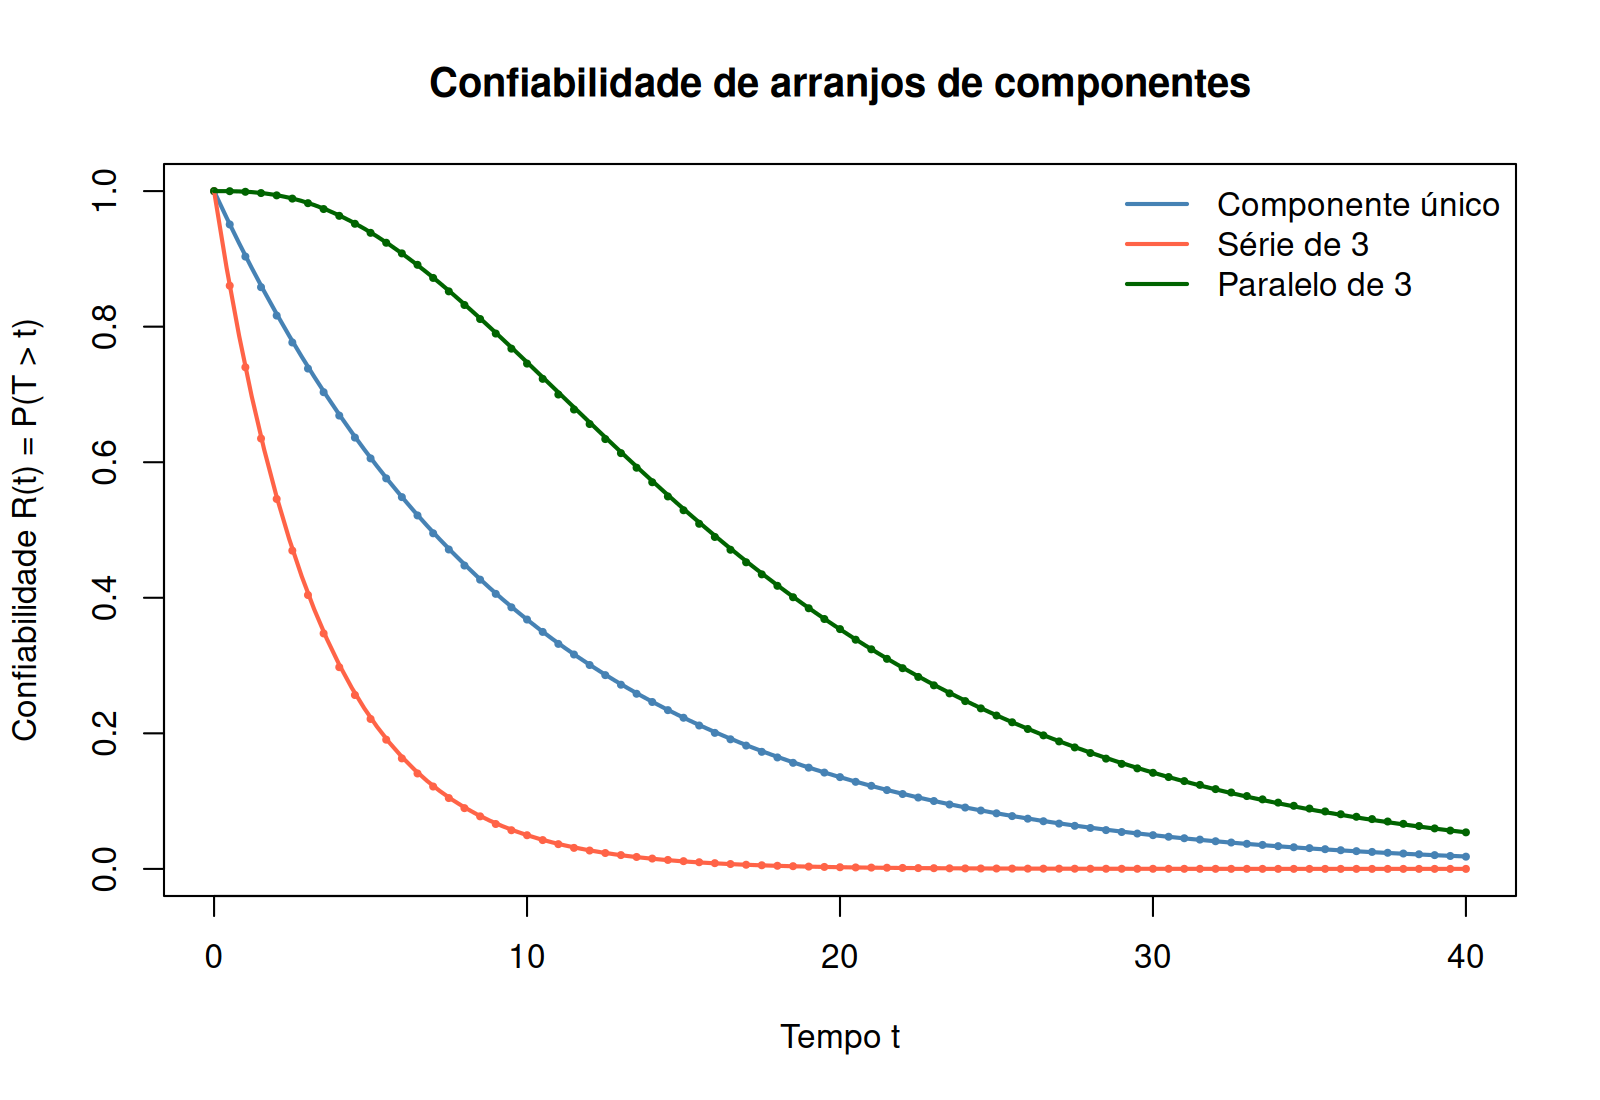
\includegraphics[width=0.8\textwidth]{secoes/07_atividade_integradora/atv_2/imagens/fig_conf_curvas.png}
	\caption{Confiabilidade $R(t)$ dos arranjos único, série e paralelo.}
	\label{fig:conf_curvas}
\end{figure}

Os valores empíricos e teóricos concordam em todos os arranjos analisados. A
comparação evidencia a relação entre custo e confiabilidade, pois a
redundância em paralelo eleva o tempo médio até a falha ao preço de mais
componentes, enquanto o arranjo em série, embora mais simples, é menos confiável
que um único componente. A hipótese de taxa de falha constante é uma
simplificação, pois na prática a chance de falha pode mudar com o tempo de uso do
componente.
